\ifdefined\included
\else
\documentclass[a4paper,11pt,twoside]{StyleThese}
\usepackage{amsmath,amssymb, amsthm}             % AMS Math
\usepackage[T1]{fontenc}
\usepackage[utf8x]{inputenc}
\usepackage{babel}
\usepackage{datetime}

\usepackage{silence}

\WarningFilter{minitoc(hints)}{W0023}
\WarningFilter{minitoc(hints)}{W0028}
\WarningFilter{minitoc(hints)}{W0030}

\usepackage{lmodern}
\usepackage{tabularx}
%\usepackage{tabular}
\usepackage{multirow}
\usepackage{xspace}

\usepackage{hhline}
\usepackage[left=1.5in,right=1.3in,top=1.1in,bottom=1.1in,includefoot,includehead,headheight=13.6pt]{geometry}
\renewcommand{\baselinestretch}{1.05}

% Table of contents for each chapter

\usepackage[nottoc, notlof, notlot]{tocbibind}
\usepackage{minitoc}
\setcounter{minitocdepth}{2}
\mtcindent=15pt
% Use \minitoc where to put a table of contents

\usepackage{aecompl}

% Glossary / list of abbreviations

\usepackage[intoc]{nomencl}
\iftoggle{ThesisInEnglish}{%
\renewcommand{\nomname}{Glossary}
}{ %
\renewcommand{\nomname}{Liste des Abréviations}
}

\usepackage{etoolbox}
\renewcommand\nomgroup[1]{%
  \item[\bfseries
  \ifstrequal{#1}{A}{Number Sets}{%
  \ifstrequal{#1}{G}{Agents Beliefs and Action Models}{%
  \ifstrequal{#1}{N}{Navigation}{%
  \ifstrequal{#1}{O}{Ontology}{%
  \ifstrequal{#1}{R}{Referring Expression Generation}{%
  \ifstrequal{#1}{Z}{Controllable and Uncontrollable Agents Task Planning}{}}}}}}%
]}

\makenomenclature



% My pdf code

\usepackage{ifpdf}

\ifpdf
  \usepackage[pdftex]{graphicx}
  \DeclareGraphicsExtensions{.jpg}
  \usepackage[pagebackref,hyperindex=true]{hyperref}
  \usepackage{tikz}
  \usetikzlibrary{arrows,shapes,calc}
\else
  \usepackage{graphicx}
  \DeclareGraphicsExtensions{.ps,.eps}
  \usepackage[dvipdfm,pagebackref,hyperindex=true]{hyperref}
\fi

\graphicspath{{.}{images/}}

%% nicer backref links. NOTE: The flag ThesisInEnglish is used to define the
% language in the back references. Read more about it in These.tex

\iftoggle{ThesisInEnglish}{%
\renewcommand*{\backref}[1]{}
\renewcommand*{\backrefalt}[4]{%
\ifcase #1 %
(Not cited.)%
\or
(Cited in page~#2.)%
\else
(Cited in pages~#2.)%
\fi}
\renewcommand*{\backrefsep}{, }
\renewcommand*{\backreftwosep}{ and~}
\renewcommand*{\backreflastsep}{ and~}
}{%
\renewcommand*{\backref}[1]{}
\renewcommand*{\backrefalt}[4]{%
\ifcase #1 %
(Non cité.)%
\or
(Cité en page~#2.)%
\else
(Cité en pages~#2.)%
\fi}
\renewcommand*{\backrefsep}{, }
\renewcommand*{\backreftwosep}{ et~}
\renewcommand*{\backreflastsep}{ et~}
}

% Links in pdf
\usepackage{color}
\definecolor{linkcol}{rgb}{0,0,0.4} 
\definecolor{citecol}{rgb}{0.5,0,0} 
\definecolor{linkcol}{rgb}{0,0,0} 
\definecolor{citecol}{rgb}{0,0,0}
% Change this to change the informations included in the pdf file

\hypersetup
{
bookmarksopen=true,
pdftitle="Planning For Both Robot and Human: Anticipating and Accompanying Human Decisions",
pdfauthor="Guilhem BUISAN", %auteur du document
pdfsubject="Thèse", %sujet du document
%pdftoolbar=false, %barre d'outils non visible
pdfmenubar=true, %barre de menu visible
pdfhighlight=/O, %effet d'un clic sur un lien hypertexte
colorlinks=true, %couleurs sur les liens hypertextes
pdfpagemode=None, %aucun mode de page
pdfpagelayout=SinglePage, %ouverture en simple page
pdffitwindow=true, %pages ouvertes entierement dans toute la fenetre
linkcolor=linkcol, %couleur des liens hypertextes internes
citecolor=citecol, %couleur des liens pour les citations
urlcolor=linkcol %couleur des liens pour les url
}

% definitions.
% -------------------

\setcounter{secnumdepth}{3}
\setcounter{tocdepth}{2}

% Some useful commands and shortcut for maths:  partial derivative and stuff

\newcommand{\pd}[2]{\frac{\partial #1}{\partial #2}}
\def\abs{\operatorname{abs}}
\def\argmax{\operatornamewithlimits{arg\,max}}
\def\argmin{\operatornamewithlimits{arg\,min}}
\def\diag{\operatorname{Diag}}
\newcommand{\eqRef}[1]{(\ref{#1})}

\usepackage{rotating}                    % Sideways of figures & tables
%\usepackage{bibunits}
%\usepackage[sectionbib]{chapterbib}          % Cross-reference package (Natural BiB)
%\usepackage{natbib}                  % Put References at the end of each chapter
                                         % Do not put 'sectionbib' option here.
                                         % Sectionbib option in 'natbib' will do.
\usepackage{fancyhdr}                    % Fancy Header and Footer

% \usepackage{txfonts}                     % Public Times New Roman text & math font
  
%%% Fancy Header %%%%%%%%%%%%%%%%%%%%%%%%%%%%%%%%%%%%%%%%%%%%%%%%%%%%%%%%%%%%%%%%%%
% Fancy Header Style Options

\pagestyle{fancy}                       % Sets fancy header and footer
\fancyfoot{}                            % Delete current footer settings

%\renewcommand{\chaptermark}[1]{         % Lower Case Chapter marker style
%  \markboth{\chaptername\ \thechapter.\ #1}}{}} %

%\renewcommand{\sectionmark}[1]{         % Lower case Section marker style
%  \markright{\thesection.\ #1}}         %

\fancyhead[LE,RO]{\bfseries\thepage}    % Page number (boldface) in left on even
% pages and right on odd pages
\fancyhead[RE]{\bfseries\nouppercase{\leftmark}}      % Chapter in the right on even pages
\fancyhead[LO]{\bfseries\nouppercase{\rightmark}}     % Section in the left on odd pages

\let\headruleORIG\headrule
\renewcommand{\headrule}{\color{black} \headruleORIG}
\renewcommand{\headrulewidth}{1.0pt}
\usepackage{colortbl}
\arrayrulecolor{black}

\fancypagestyle{plain}{
  \fancyhead{}
  \fancyfoot{}
  \renewcommand{\headrulewidth}{0pt}
}

%\usepackage{MyAlgorithm}
%\usepackage[noend]{MyAlgorithmic}
\usepackage{algorithm}
\usepackage[noend]{algpseudocode}
\usepackage{comment}
\usepackage[ED=EDSYS-Robo, Ets=INSA]{tlsflyleaf}
%%% Clear Header %%%%%%%%%%%%%%%%%%%%%%%%%%%%%%%%%%%%%%%%%%%%%%%%%%%%%%%%%%%%%%%%%%
% Clear Header Style on the Last Empty Odd pages
\makeatletter

\def\cleardoublepage{\clearpage\if@twoside \ifodd\c@page\else%
  \hbox{}%
  \thispagestyle{empty}%              % Empty header styles
  \newpage%
  \if@twocolumn\hbox{}\newpage\fi\fi\fi}

\makeatother
 
%%%%%%%%%%%%%%%%%%%%%%%%%%%%%%%%%%%%%%%%%%%%%%%%%%%%%%%%%%%%%%%%%%%%%%%%%%%%%%% 
% Prints your review date and 'Draft Version' (From Josullvn, CS, CMU)
\newcommand{\reviewtimetoday}[2]{\special{!userdict begin
    /bop-hook{gsave 20 710 translate 45 rotate 0.8 setgray
      /Times-Roman findfont 12 scalefont setfont 0 0   moveto (#1) show
      0 -12 moveto (#2) show grestore}def end}}
% You can turn on or off this option.
% \reviewtimetoday{\today}{Draft Version}
%%%%%%%%%%%%%%%%%%%%%%%%%%%%%%%%%%%%%%%%%%%%%%%%%%%%%%%%%%%%%%%%%%%%%%%%%%%%%%% 

\newenvironment{maxime}[1]
{
\vspace*{0cm}
\hfill
\begin{minipage}{0.5\textwidth}%
%\rule[0.5ex]{\textwidth}{0.1mm}\\%
\hrulefill $\:$ {\bf #1}\\
%\vspace*{-0.25cm}
\it 
}%
{%

\hrulefill
\vspace*{0.5cm}%
\end{minipage}
}

\let\minitocORIG\minitoc
\renewcommand{\minitoc}{\minitocORIG \vspace{1.5em}}

\usepackage{multirow}
%\usepackage{slashbox}

\newenvironment{bulletList}%
{ \begin{list}%
	{$\bullet$}%
	{\setlength{\labelwidth}{25pt}%
	 \setlength{\leftmargin}{30pt}%
	 \setlength{\itemsep}{\parsep}}}%
{ \end{list} }

\theoremstyle{definition}
\newtheorem{definition}{Definition}
\renewcommand{\epsilon}{\varepsilon}

% centered page environment

\newenvironment{vcenterpage}
{\newpage\vspace*{\fill}\thispagestyle{empty}\renewcommand{\headrulewidth}{0pt}}
{\vspace*{\fill}}

\usepackage{tablefootnote}

\theoremstyle{plain}
\newtheorem{constraint}{Constraint}[section]

\algnewcommand\algorithmicforeach{\textbf{for each}}
\algnewcommand\algorithmicin{\textbf{in}}
\algdef{S}[FOR]{ForEach}[2]{\algorithmicforeach\ #1\ \algorithmicin\ #2\ \algorithmicdo}

\usepackage{listings}
\lstdefinestyle{customPlan}{
  language=C,
  commentstyle=\itshape\color{green!25!black},
}
\usepackage{pdfpages}

\sloppy
\begin{document}
\setcounter{chapter}{1} %% Numéro du chapitre précédent ;)
\dominitoc
\faketableofcontents
\fi

\chapter{Coplanning for navigation}
\minitoc

\section{Introduction}
In a lot of human robot interaction scenarios, the robot has to move in the environment to accomplish its task. It can either be that the task cannot be done in the direct vicinity of the robot or that the task itself is to move elsewhere. For example in the MuMMER project, a Pepper robot in a mall has to give direction instructions to guide a human to their wanted location. The robot is also able to point to visible landmarks to locate the beginning of the route (\textit{e.g.} saying \textit{"Take these stairs, then take the corridor on your right and the shop will be on your left" while pointing to the stairs}). However, some obstacles in the proximity of the robot and the guided human can prevent them to see the pointed landmarks, or a corridor crossing can be hidden, making the route description one step longer than it should be. Thus, to perform the task of route guiding more efficiently, the robot might decide to move.
In the Spencer project, another robot has to guide people to their gate in the Schipol airport. Here, the robot will navigate all the way from the starting point to the final destination while ensuring the human is actually following it, but also has to avoid other pedestrians. In this example, the navigation of the robot is a main part of the task.
In both example, the robot has to make plan its motion such as the physical and psychological safety of surrounding humans are ensured. However, not taking into account the motion of these humans during the planning process may lead to suboptimal trajectories or even deadlock.
We propose in this chapter to, after a survey of related works, present a navigation planner algorithm taking into account both the robot and the human, then to show how this approach can be used to enhance mutual manifestness and improve efficiency in a narrow corridor crossing scenario through a user study, and finally report some extension made to the approach to include humanoid robots, flying drone and to estimate the progression of the navigation task. 

\section{Related Work}
\subsection{Human-Aware Robot Navigation}
The aim of robot navigation is to make the robot base move from one place to another while avoiding static and moving obstacles. However, when the robot has to move in an environment where humans are evolving other constraints must be added. The robot must not only avoid the humans, as any other moving obstacle, to ensure their physical safety (not harming them), but also take into account their psychological safety (not stressing or frightening them) \cite{sisbot_human_2007}, \cite{kruse_human-aware_2013}. In order to respect these constraints several methods have been used. The first largely used is based on costmap exploration. Based on the robot known humans and obstacles in the environment a grid is built, where each cell has a cost representing places the robot should avoid to pass through. Then, given a start and an end points, a planner can explore this grid and try to minimize the cost along the trajectory (\cite{sisbot_human_2007}, \cite{lu_towards_2013}). These approaches are usually pretty efficient but since a whole grid can take time to compute, they can perform poorly in dynamic environments.

Another approach is to use the social force model \cite{helbing_social_1995}. A robot trajectory is computed based on repulsive or attractive force fields set on humans, obstacles and goal \cite{ferrer_robot_2013}. This gives good results in open environments but the trajectories can be erratic in confined environment with a lot of obstacles and humans because of the diverging "forces" applied. Moreover, by only considering the robot plan, these planners return no solution if the robot and the human must cross each other in a narrow corridor where the human is centered leaving no place for the robot to go. This is why we need a planner able to \textit{infer} that the human can move to one side of the corridor allowing the robot to cross on the other side.

In their work, Kuderer et al. use social force model to both compute the robot trajectories and predict the nearby human ones \cite{kuderer_feature-based_2012}. However, the resulting human trajectories are more reactions to robot motion than coplanning solutions.

To overcome this limitation, Khambhaita \& Alami proposed a navigation planner based on an optimization scheme. In this approach the trajectories of the robot and of the nearby humans are optimized together at real time to create, at position control rate, a conavigation solution \cite{khambhaita_viewing_2017}. This ensures that at all time it exists for the humans a solution to go to their known goal, and that this solution is optimal regarding a different set of constraint based on human models.

Although, even if the robot computes an optimal solution for the human and itself, it is pointless if it cannot communicate or show this solution to the human (\textit{e.g.} either it plans to go to the left or the right of the corridor, so the human can either accept or decline this plan). Thus, the robot must also try to make its intention clear \cite{pacchierotti_evaluation_2006}. This ability of a robot to exhibit its future actions is called legibility. A legible robot will have its future actions and goals inferred quicker \cite{dragan_legibility_2013}, which is crucial in entangled tasks such as crossing in a narrow corridor. For navigation, legibility can be increased either by changing the robot speed along the trajectory \cite{kruse_legible_2012} or by modifying its trajectory \cite{khambhaita_viewing_2017}.

In a broader sense, the changes in an agent's own behavior in order to make easier the interaction with another agent are called coordination smoothers \cite{vesper_minimal_2010}. We claim that a robot should exhibit some coordination smoothers when interacting with a human to increase its usability. Moreover, all the coordination smoothers are not equal, as some can bring more information thant other. A simple blinking light and beeping sound when the robot is moving are conveying less information than turn signals for example. In our case, since we deal with anthropomorphic robots, we can try to make even more efficient coordination smoothers by using what can be identified as the head of the robot.

\subsection{Communicating Intents Via the Robot Gaze} \unsure{Cette subsection n'a peut-être rien à faire ici...}
Some robots have a movable part that can be identified as an head, and often contains camera or similar devices that can be recognized eyes. the resulting robot \textit{gaze} has already been used to effectively increase the user attention and engagement \cite{mutlu_storytelling_2006}, \cite{zaraki_designing_2014}. Moreover, the robot gaze has also been shown useful in navigation to indicate turning intentions \cite{lu_towards_2013}, \cite{may_show_2015}, and thus increase legibility.

Besides, in intricate collaborative activities, each agent must show to the other one that they are aware of their presence and actions. Pacherie defines it as the mutual manifestness: \textit{each subject must be aware, in some sense, of the event as an event that is present to both; in other words the fact that both are attending to the same object or event should be open or mutually manifest} \cite{pacherie_phenomenology_2011}. Thus, it is interesting to know if in intricate human robot navigation tasks, making the robot show mutual manifestness increase the efficiency of the task.



\section{The Human Aware Timed Elastic Band}
The only work to our knowledge being able to, in real time, plan trajectories for the robot and the humans surrounding it, is the \textit{Human Aware Timed Elastic Band} \cite{khambhaita_viewing_2017}. Thus, we used it as the backbone of our work, and made several contributions around it.

\subsection{General scheme}
The human aware timed elastic band algorithm is based on the timed elastic band (TEB) approach from Rosmann et al. \cite{rosmann_efficient_2013}. This approach is a local optimization problem where the successive positions $(x_i, y_i) \in \realset$ and orientations $\theta_i \in S^1$ of the robot along with the time steps $\Delta T_i \in \realset$ between each consecutive poses are optimized to minimize a multi criteria cost function up to a fixed length horizon $n \in \intset$. To put it otherwise, the elastic band trajectory of the robot is represented by its poses: 
\[Q = \{\textbf{s}_i\}_{i=0..n} with \textbf{s}_i = [x_i, y_i, \theta_i]^T\] to which are added the time intervals between two consecutive poses: \[\tau = {\Delta T_i}_{i=0..n-1}\] Resulting in the \textit{time elastic band} \[B := (Q, \tau)\] having to be optimized to minimize the cost function $f(B)$ to get the optimal trajectory \[B^* = \mathop{\mathrm{argmin}}_B\,f(B)\]
This function takes the form of a multi criteria weighted sum cost function which can be rewritten as: \[ f(B) = \sum_{k} \gamma_k f_k(B) \] where $\gamma_k \in \realset$ are weights allowing the designer to balance the importance between cost functions $f_k$.

This planner has been integrated has a local planner in the ROS architecture. Provided with a global plan (often generated with an A* algorithm) of the long trajectory, the local planner generates short term plans (up to several meters), avoiding static and dynamic obstacles (both known by the global planner and discovered with the robot sensor during the navigation) and minimizing the trajectory duration. In addition, the local planner is responsible for generating the speed command at position control rate (around 10 Hz usually). TEB does it by optimizing the local trajectory and computing the wanted robot speed from the first two poses and the time interval between them. Moreover, if the optimization process takes too long, the length horizon of the global trajectory on which the local optimization is performed is reduced, and increased if the optimization time is satisfactory.

In the human aware timed elastic band approach, multiple timed band are considered. In addition to the robot band $\robotband$ represents the robot trajectory, it also considers multiple human bands $B_{\mathcal{H}_k}$ with $k in \intset$ the number of humans in vicinity of the robot. For simplicity purpose, in this thesis we will only consider one human in the vicinity of the robot, and thus one human band $\humanband$. However, the approach has been shown working successfully up to three humans.
Moreover, the weighted-sum cost function becomes:
\[f(\robotband, \humanband) = \sum_a \gamma_a f_a(\robotband) + \sum_b \gamma_b f_b(\humanband) + \sum_c \gamma_c f_c(\robotband, \humanband) \]

where $fa$, $fb$ and $fc$ represent respectively cost functions associated with robot trajectory constraints, human trajectory constraints and human-robot social constraints. Then, the optimization process consist in finding the optimal robot and human trajectories $\robotband, \humanband$ such as:
\[\{\robotband^*, \humanband^*\} = \mathop{\mathrm{argmin}}_{\{\robotband, \humanband\}}\,f(\robotband, \humanband)\]





\subsection{Constraints}
In this optimization scheme, all the constraints are represented as cost in the function. Thus, there is no \textit{hard constraints}, but using the weight of each one, we are able to prioritize some over the others. Moreover, when a trajectory has been optimized, before being executed, the local planner checks that it respects all the defined hard constraints (kinodynamic constraints and obstacles separation).

The new formulation of Khambhaita et al. allows to separate the constaints into three categories:
\begin{itemize}
\item Robot trajectory constraints: these constraints represent the robot kinodynamic constraints (non holonomic, maximum speed, maximum acceleration) as well as preventing the robot trajectory to differ too much from the global plan. They are presented in \cite{rosmann_efficient_2013}.
\item Human trajectory constraints: these constraints represent the human kinodynamic constraints and prevent them to differ too much from the global trajectory. They are the same as the robot ones, but their parameters (\textit{e.g.} maximum speed threshold) must not be set by the designer but evaluated by the robot during the evaluation.
\item Human-robot social constraints: these constraints represent how the human and robot trajectory must interact with each other. Khambhaita et al. presneted the \textit{safety} constraint, ensuring a sufficient distance between the robot and the human; the \textit{directional constraint} discouraging trajectories where the robot and the human move straight to each other; and the \textit{time-to-collision} (TTC) constraint, preventing the robot and the human to adopt speed which, if maintained, would lead to a collision. The latter will be detailed in what follows as it was studied more in depth through a user study.
\end{itemize}

It worth noting that different weights can be set for each constraint, and that they can be adjusted dynamically during the navigation. Moreover, by setting different weight between the robot and the human for the constraint preventing to move away from the global plan, we can adjust the \textit{stiffness} of the trajectories, thus allowing one agent or the other to elongate their trajectory, taking more or less effort into the collaborative navigation.

\section{Evaluating enhanced mutual manifestness in a crossing scenario}
In this section we present an user study aiming at assessing the pertinence of using a conavigation planner in a situation where a human and a robot must cross each other in a narrow corridor. This task of crossing in narrow corridor is challenging as both agents start in the center of either end of the corridor, and there is no way for one agent to find a way if the other agent does not move to the other side. Thus, we state that not only coplanning is required to find a plan reaching the other end of the corridor (by planning that the other agent will also cooperate and move on one side), but showing intentions and awareness of the other agent is crucial for the interaction to unfold without trouble.

\subsection{Robot behavior design}
For this user study we were particularly interested in finding if and how navigation coplanning would lead to higher mutual manifestness and to higher efficiency in crossing.
To do so, we designed a robot behavior using the HATEB navigation planner.
In their work Kambhaita et al. showed that during a narrow crossing the robot is able to plan that the human and the robot will choose opposite sides of the corridor. But if the robot shows its plan when it faces the human, they would have little time to react, and might also move to the same side as the robot, needing negotiation and replanning, reducing the overall efficiency of the crossing. The robot must thus, show the plan (\textit{i.e.} the plan trajectory, or here, the side of the corridor it plans to take) early in the crossing.
By reducing the TTC constraint function threshold and increasing its weight, we discourage trajectories where the robot and the human are facing each other. Thus, if the robot trajectory stiffness is lower than the human one, the robot will move to the chosen side of the corridor early in the trajectory as shown in Fig.~\ref{ttc_explanations}.


\begin{figure}[hbtp]
\centering
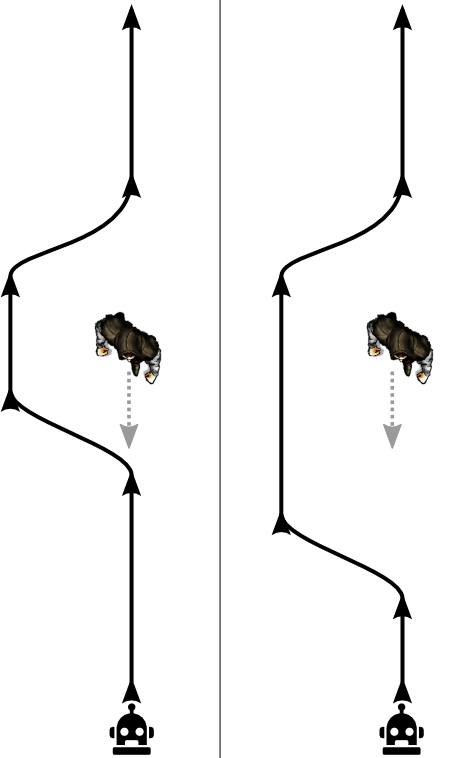
\includegraphics[scale=0.4]{figures/chapter2/condition_1_proactivity_shrink.png}
\caption{Influence of the modification of the TTC constraint cost weight on the trajectory. On the left, the weight is low, the robot will show the side and avoid the human at the last moment. On the right, the weight is high, the robot will show the chosen side and avoid the human much earlier.}
\label{ttc_explanations}
\end{figure}

Moreover, as stated before \unsure{maybe move the gaze stuff from related work to here?} several papers show that using the \textit{head} of a robot can significantly improve legibility and mutual manifestness. Thus, we also chose to make the robot look at its future planned trajectory as shown in Fig.~\ref{head_gaze_behavior}. This is possible thanks to the HATEB algorithm which, unlike many other local planner only publishing  speed commands \improvement{Adds ref to DWA for example ?}, also publishes a precise short-term trajectory. Finally, to show the robot awareness of the human presence, we made it \textit{glance} at the human twice when they enter a large and a small radius circle.

\begin{figure}[hbtp]
\centering
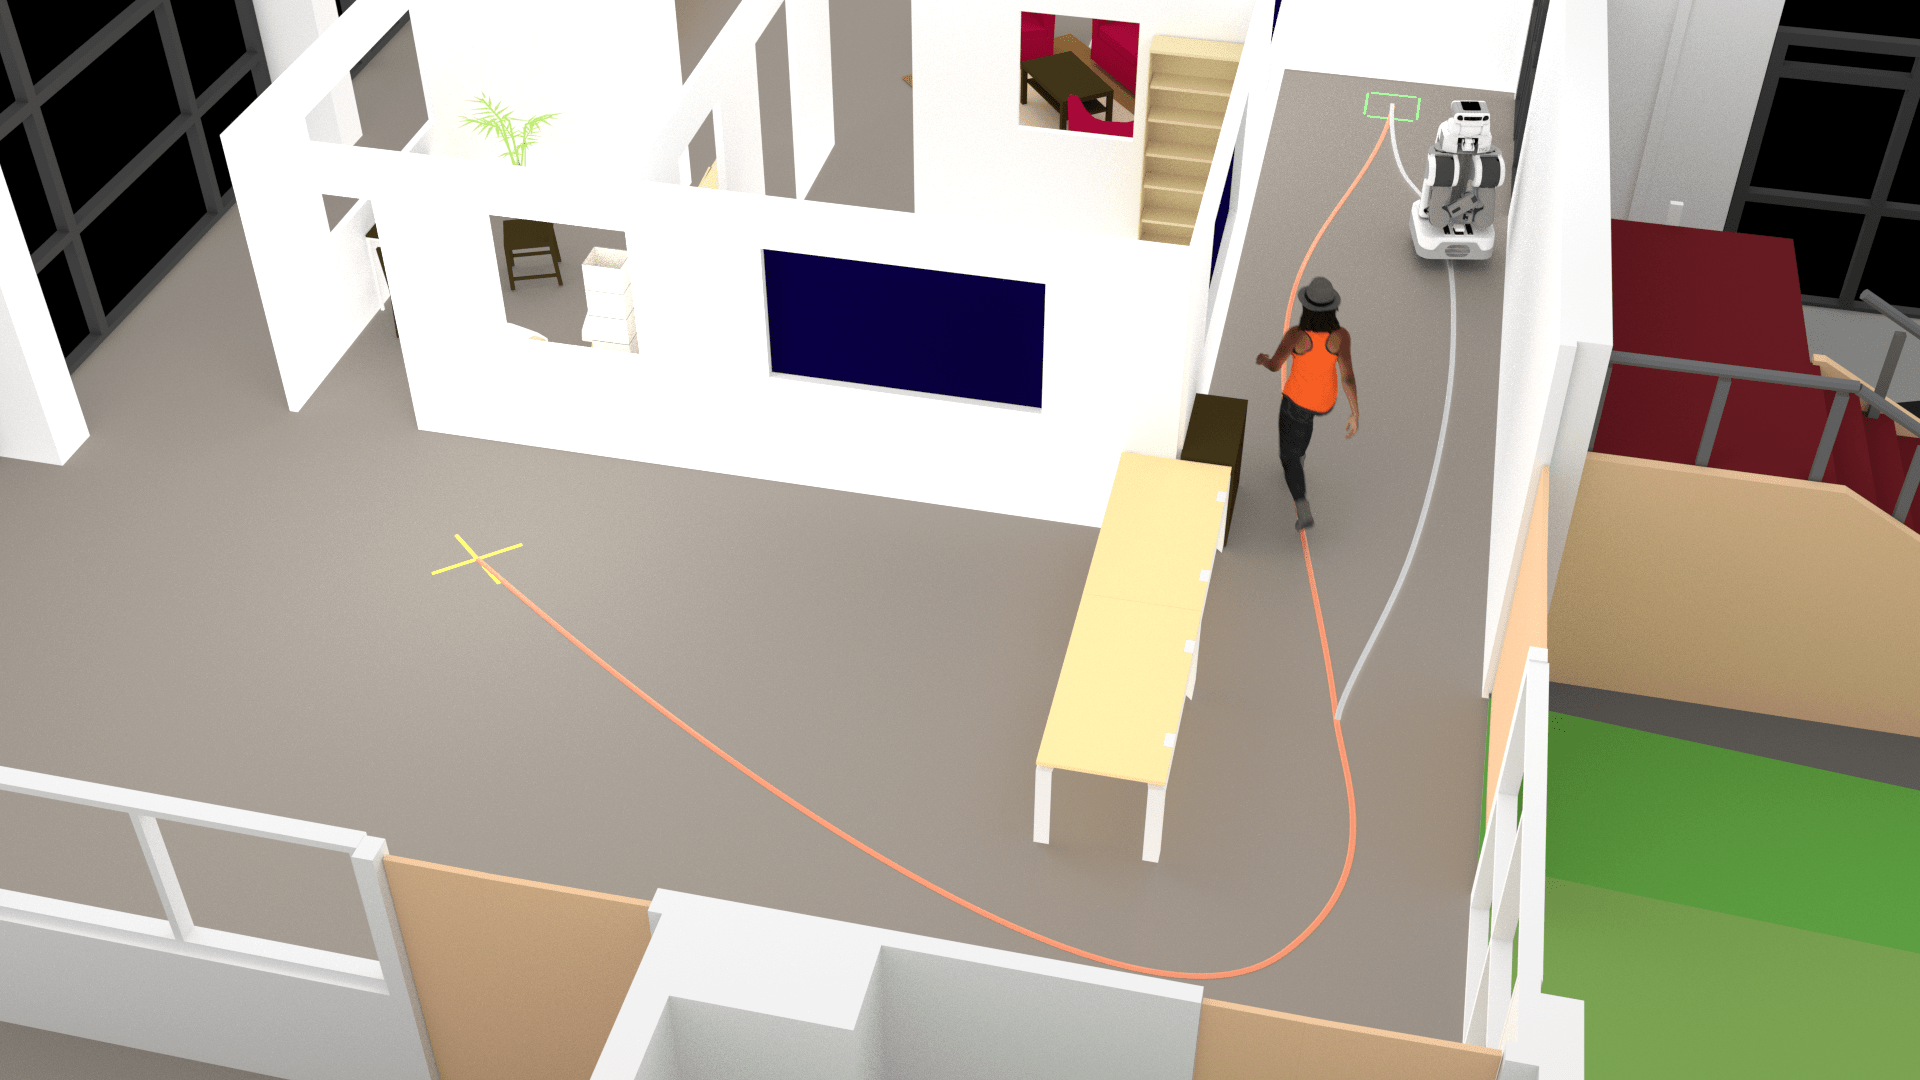
\includegraphics[scale=0.4]{figures/chapter2/expe_human-min.png}
\caption{Behavior implemented for the robot head. The robot \textit{looks} at a point placed at its planned position X seconds in the future and h meters above the ground.}
\label{experiment_adream}
\end{figure}

\subsection{User study protocol}

\begin{figure}[hbtp]
\centering
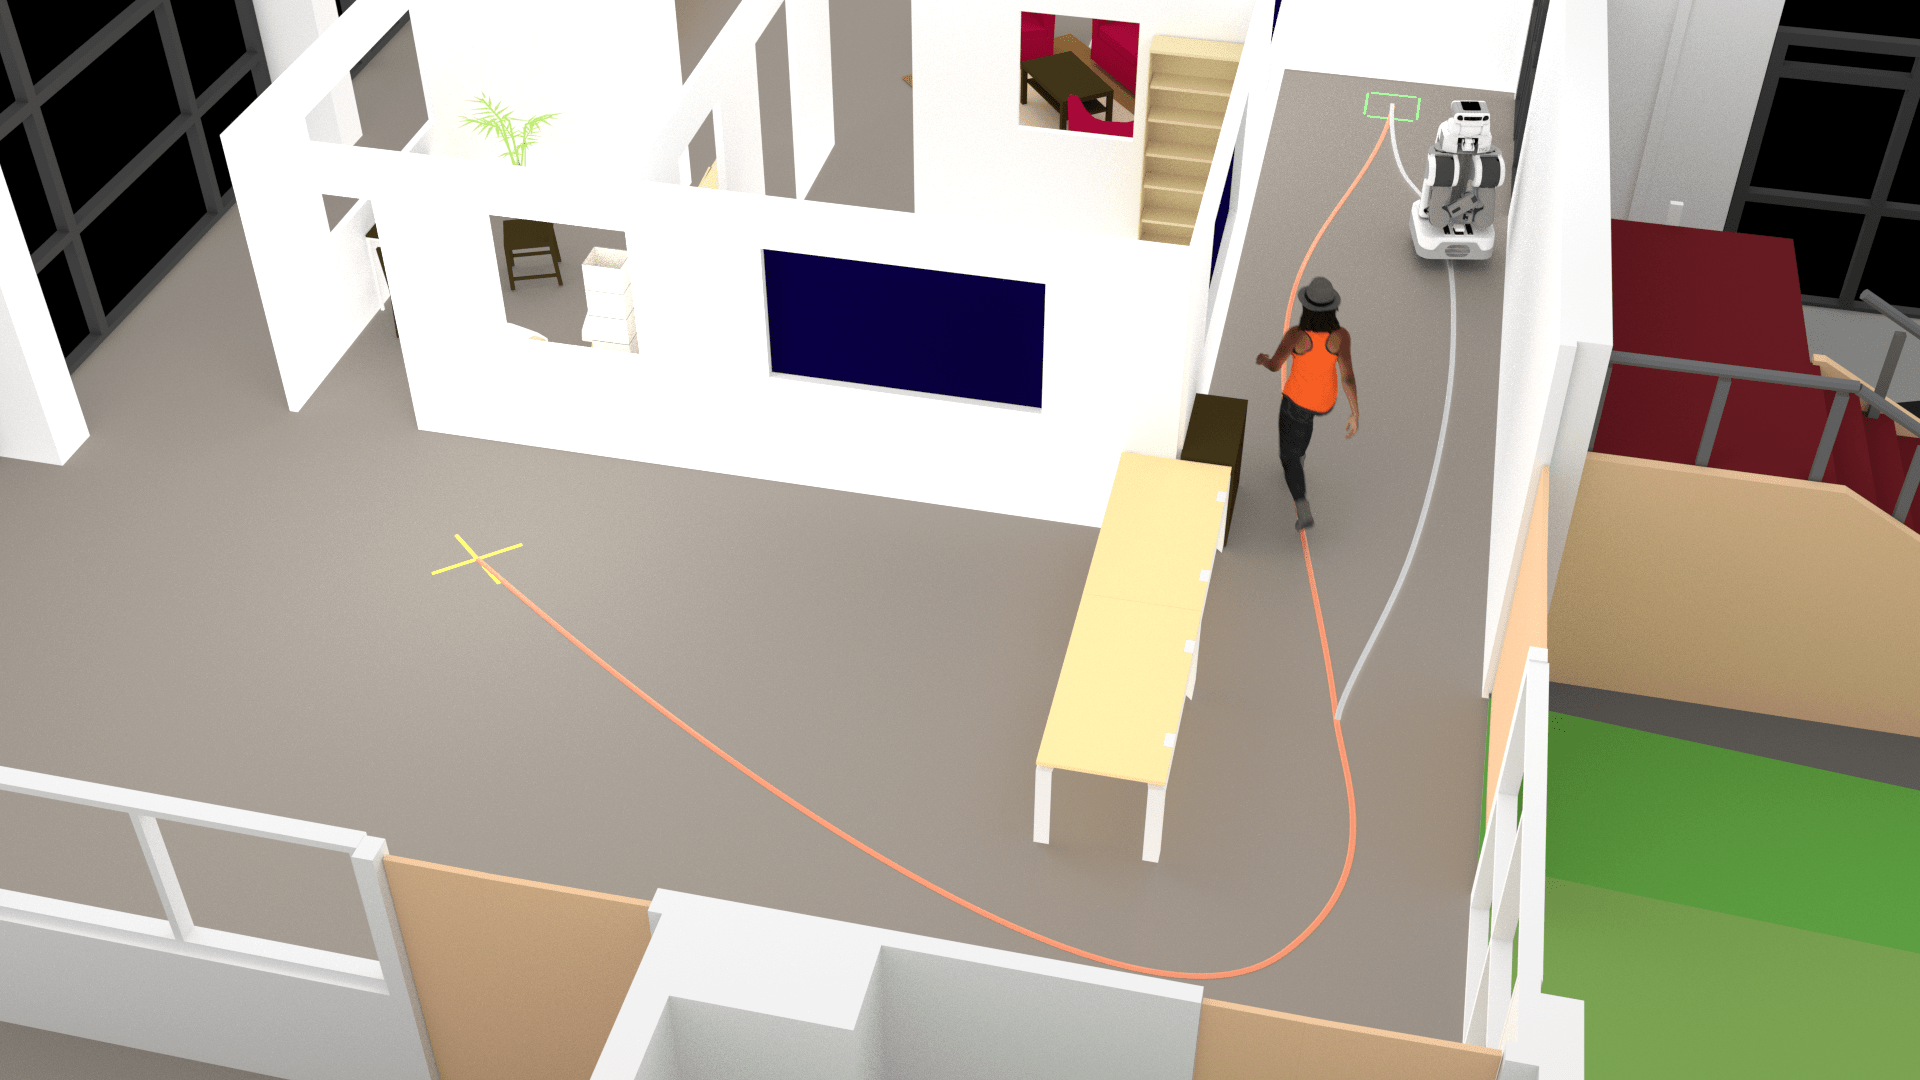
\includegraphics[scale=0.4]{figures/chapter2/expe_human-min.png}
\caption{The  study  environment.  The  participant  had  to  go  from  the  yellow  cross  marked  on  the  ground  to  the  green  square  also  marked  on  the  ground,which was the robot starting point. Crossing occurred roughly in the area where the robot and participant are on the picture. Trajectories are displayed on the picture for example only and where not marked on the ground or suggested by the experimenters at any time.}
\label{head_gaze_behavior}
\end{figure}

\subsubsection{Objective}
The aim of this study is to evaluate the impact of the TTC cost constraint and head behavior on usability. We designed an user study where actual individuals have to walk through a corridor facing a fully autonomous navigating robot. The afore-explained robot behavior was used. We measured the quality of the interaction between the robot and the human with both objective (visual behavior) and subjective data. The subjective evaluation was based on three dimensions: (1) perceived efficiency of the robot navigation, (2) user satisfaction and (3) situation awareness.

\subsubsection{Participants}
We recruited a total of 28 participants (12 males and 18 females) aging from 21 to 41 (mean: 27.32, SD: 4.13). All 28 participants had never used or interacted with a PR2 for navigation tasks, and had a neutral or good vision of robotics (mean: 5.96 over a 7 points Likert scale, SD: 1.07). This research complied with the tenets of Declaration of Helsinki. Informed consent was obtained from each participant.

\subsubsection{Material}
A Willow Garage PR2 robot, at its lower spine position was used in this experiment. The robot measured 1.33 meters from ground to top. The entire robot can be considered as anthropomorphic and possesses a two degrees of freedom head integrating cameras resembling eyes.

The participant position was tracked using an Optitrack motion capture system, tracking a worn solid headband. This system allowed the robot to track the human anywhere in the room, without looking at them.

The experiment was conducted in a L-shaped corridor (Fig.~\ref{experiment_adream}). The participant and the robot started from opposite side of the corridor. The participant had to walk 6 meters before entering the long straight corridor part and seeing the robot, then walk 13 meters.

We used a \textit{ETG 2w} eyetracker from SMI to collect the eye movement data of the participant. It is a portable device, allowing, after a short calibration process, to track the user gaze, and measuring where the user looks at. The data were analyzed using the \textit{BeGaze 3.6} software from SMI.

Three questionnaires were used to collect the subjective measures.
\begin{itemize}
\item PeRDITA: 
\end{itemize}	

\subsubsection{Experimental design}

\subsubsection{Study procedure}

\subsubsection{Measures}

\subsection{Results}

\subsection{Discussion}

\section{Extending HATEB}
\subsection{Adapting HATEB to other robots}

\subsection{Using the estimated time to goal to measure the execution of the planned trajectory}

\section{Conclusion}

\ifdefined\included
\else
\bibliographystyle{acm}
\bibliography{These}
\end{document}
\fi
